%Este trabalho está licenciado sob a Licença Atribuição-CompartilhaIgual 4.0 Internacional Creative Commons. Para visualizar uma cópia desta licença, visite http://creativecommons.org/licenses/by-sa/4.0/deed.pt_BR ou mande uma carta para Creative Commons, PO Box 1866, Mountain View, CA 94042, USA.

\chapter{Perceptron Multicamadas}\label{cap_mlp}
\thispagestyle{fancy}

\section{Modelo MLP}\label{cap_mlp_sec_modelo}

Uma Perceptron Multicamadas (MLP, do inglês, \textit{Multilayer Perceptron}) é um tipo de Rede Neural Artificial formada por composições de camadas de perceptrons. Consulte a Figura \ref{cap_mlp_sec_modelo}.

\begin{figure}[H]
  \centering
  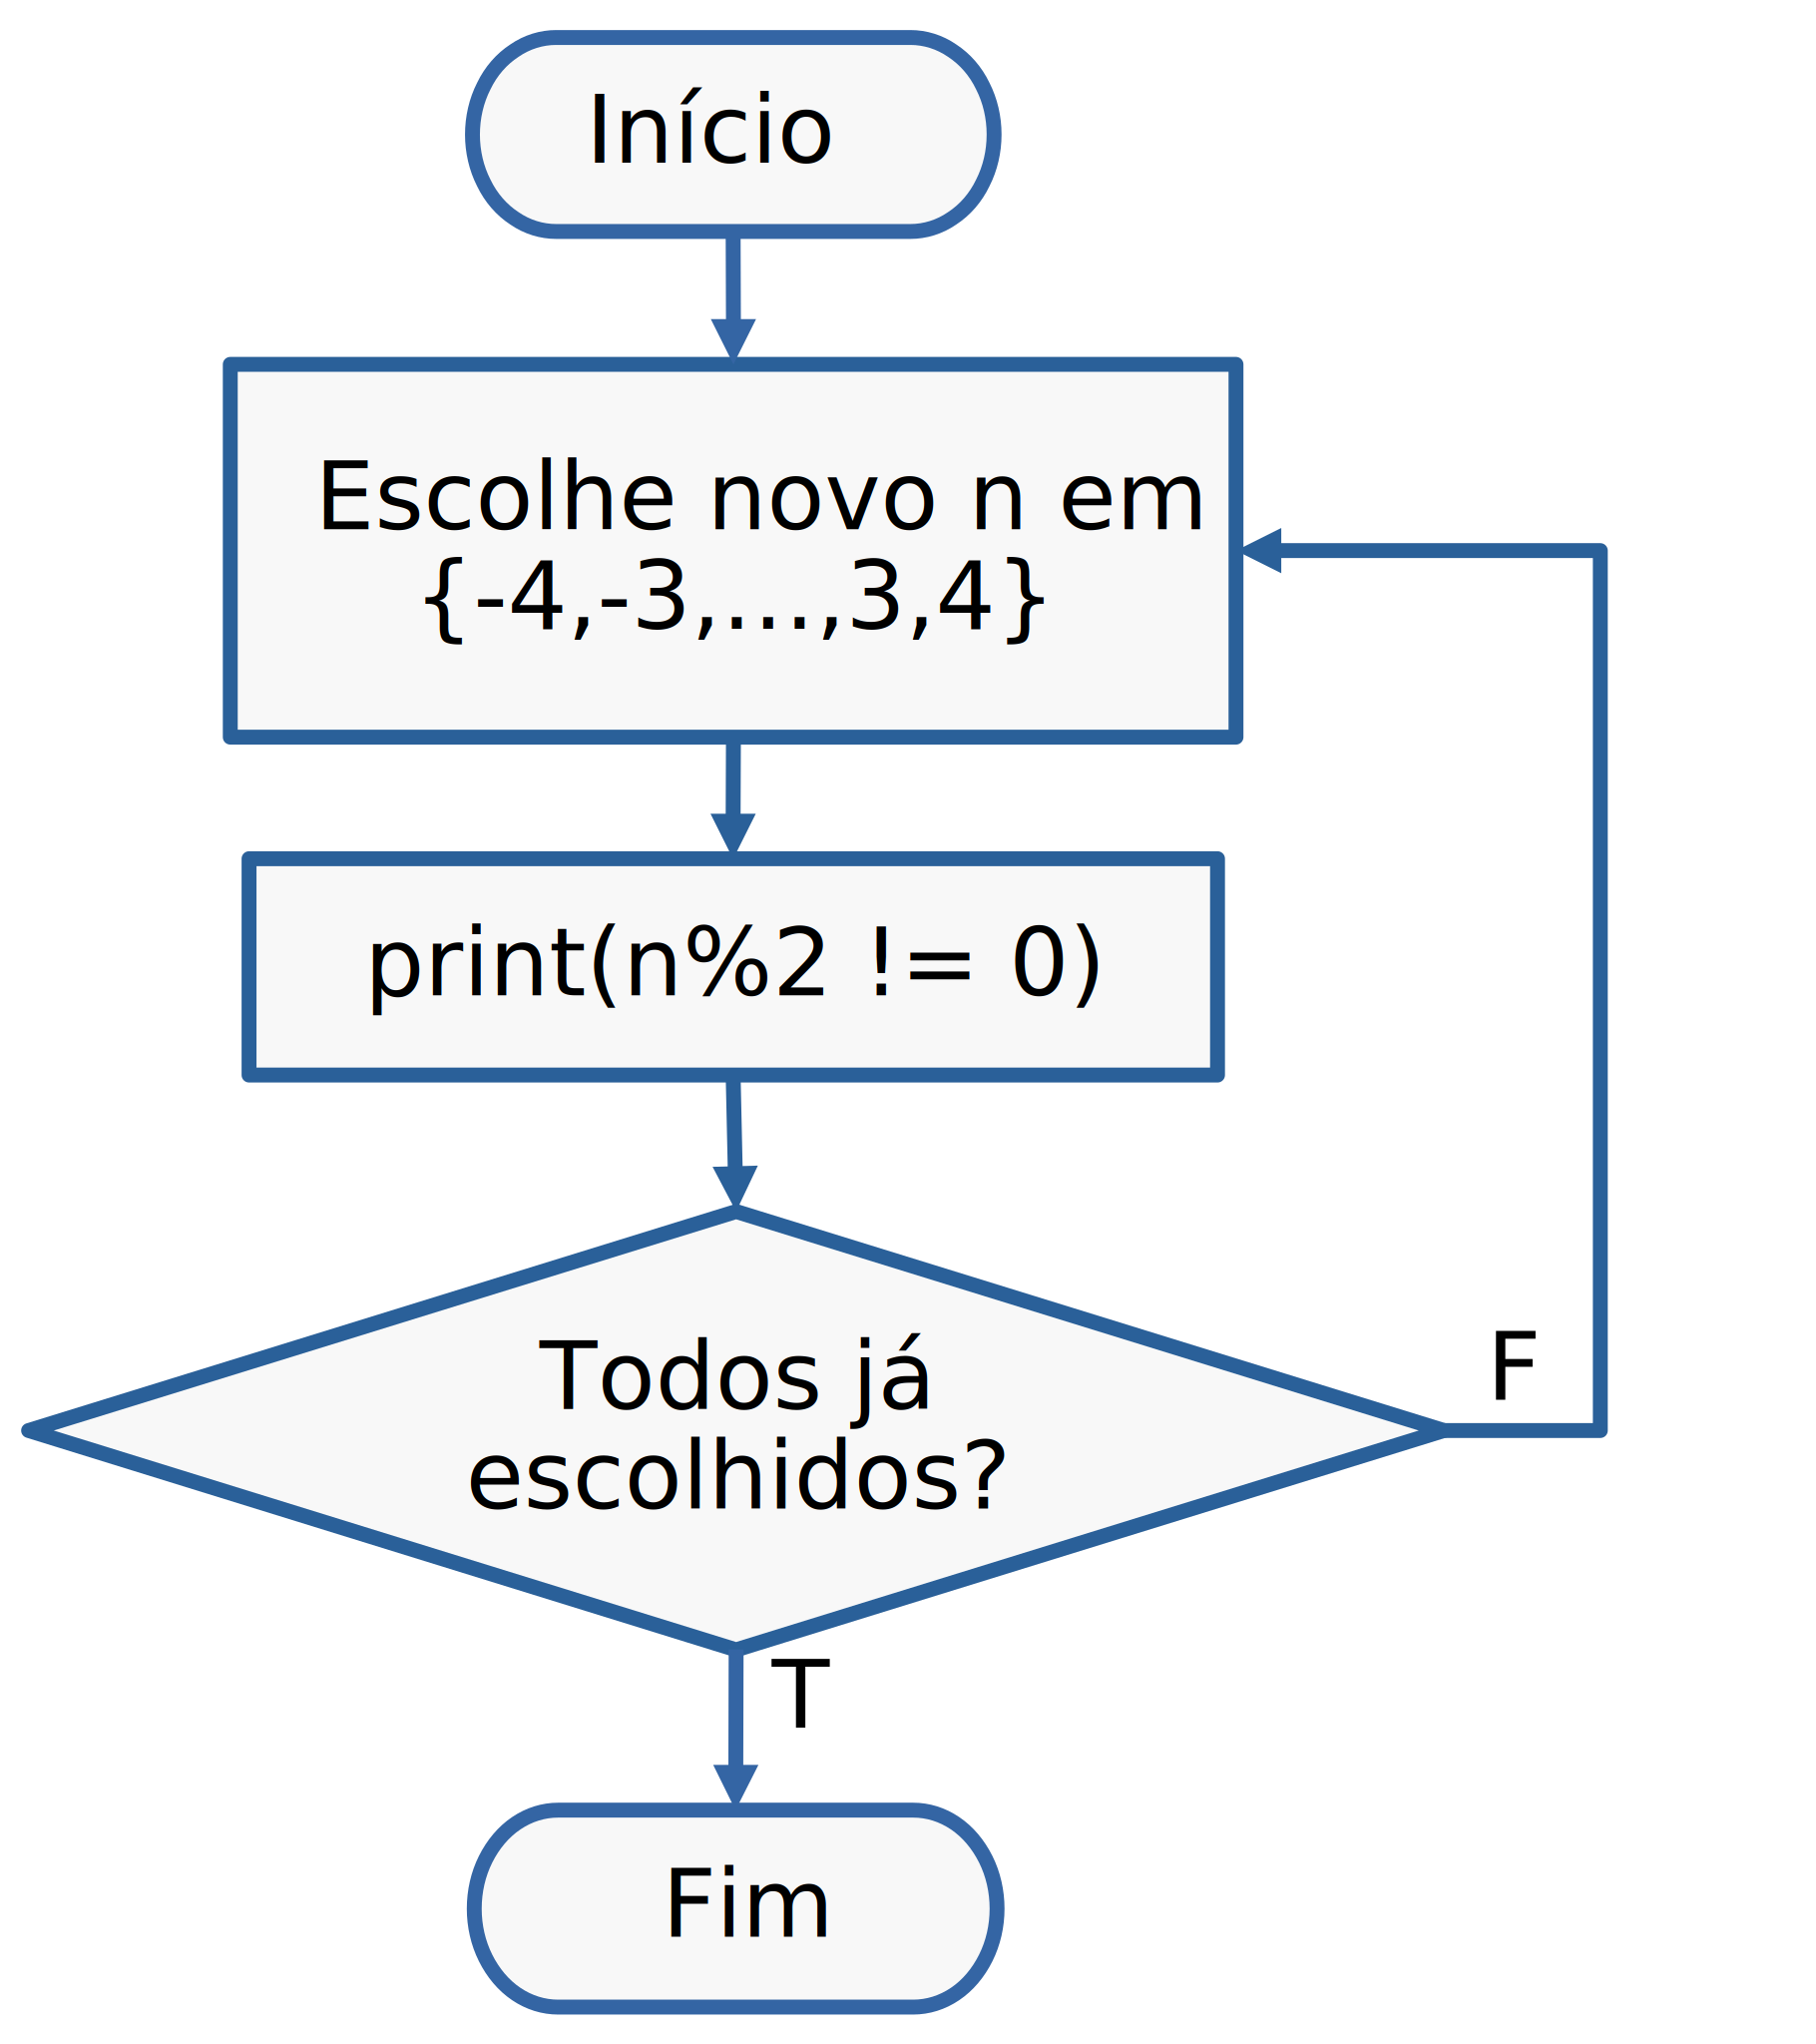
\includegraphics[width=\textwidth]{./cap_mlp/dados/fig_mlp/fig}
  \caption{Estrutura de uma rede do tipo Perceptron Multicamadas (MLP).}
  \label{fig:cap_mlp_sec_modelo:fig:mlp}
\end{figure}

Denotamos uma MLP de $n$ camadas por
\begin{align}
  \pmb{y} = \mathcal{N}\left(\pmb{x}; \left(W^{(l)}, \pmb{b}^{(l)}, f^{(l)}\right)_{l=1}^{n}\right),
\end{align}
onde $\left(W^{(l)}, \pmb{b}^{(l)}, f^{(l)}\right)$ é a tripa de pesos, bias e função de ativação da $l$-ésima camada da rede, $l=1, 2, \dotsc, n$.

A saída da rede é calculada por iteradas composições das camadas, i.e.
\begin{equation}
  \pmb{a}^{(l)} = f^{(l)}\underbrace{\left(W^{(l)}\pmb{a}^{(l-1)} + \pmb{b}^{(l-1)}\right)}_{\pmb{z}^{(l)}},
\end{equation}
para $l= 1, 2, \dotsc, n$, denotando $\pmb{a}^{(0)} := \pmb{x}$ e $\pmb{a}^{(n)} := \pmb{y}$.

\subsection{Algoritmo de Treinamento}

[[tag::construcao]]

\subsection{Aplicação: Problema de Classificação XOR}

[[tag::construcao]]

\subsection{Exercícios}

[[tag:construcao]]


\section{Aplicação: Aproximação de Funções}

[[tag::construcao]]

\subsection{Exercícios}

[[tag::construcao]]

\section{Aplicação: Resolução de EDOs}

[[tag::construcao]]

\subsection{Exercícios}

[[tag::construcao]]

\section{Aplicação: Resolução de EDPs}

[[tag::construcao]]

\subsection{Exercícios}

[[tag::construcao]]
